
{\actuality} Астрометрические исследования карликовых звезд различных типов в ближайшем окружении Солнца являются одной из актуальнейших задач, и к этому ведут многие предпосылки. Стоит уточнить, что в различных исследованиях радиус ближайшего окружения варьируется от 10 до 100 пк, но зачастую даже в одном проекте размер исследуемой области Галактики на разных этапах может расти или сокращаться в зависимости от поставленных задач.  В данной работе в основном будет идти речь о некотором усредненном значении в 50 пк, если не будет указано иное. Исследования звездного населения ближайших Солнечных окрестностей важно само по себе. В человеческой природе в первую очередь изучать то, что его окружает, и затем продвигаться дальше. И в контексте астрономии этот принцип работает наилучшим образом. В стремлении сформировать наиболее полную и объективную картину ближайшего окружения необходимы сбор и обработка большого объема статистической информации о различных типах звезд, населяющих его. Статистическая информация дает информацию о фундаментальных закономерностях и корреляциях различных характеристик, что в свою очередь позволяет формировать теории формировании и эволюции данной области, а через экстраполяцию дает возможность строить гипотезы о строении Галактики в общем. Интерес к построению и уточнению моделей Галактики и важность в данном ключе исследований Солнечных окрестностей находят отражения в целом комплексе работ (например, Зеновине и др., 2015, Сендерс, Бинней, 2015).

Как показывают результаты наблюдений космической программы Gaia, абсолютное большинство звездного населения околосолнечной области составляют различные типы карликов (см. рис. 1). Проблему нехватки наблюдений и статистических данных о звездах низкой светимости, а также важность  формирования по этим данным эмпирических соотношений и теоретической базы выделяют во многих работах.  В частности, большой научный интерес в отношении карликов представляют уточнения зависимостей <<масса "--- светимость>> (Бенедикт и др, 2016) и <<масса "--- радиус>> (Жоу и др,2014 ) и построение в согласии с этими зависимостями физических моделей маломассивных звёзд (Торрес, 2013; Спада и др., 2013). Отмечается, что в отличие от звезд солнечных и более масс, для которых существующие теории строения находят соответствие с наблюдаемыми данными, аналогичные модели для маломассивных объектов являются гораздо более несовершенными (см., например, Спада и др., 2013). Уже упомянутые эмпирические закономерности могут служить тестами моделей строения звезд и их атмосфер, и  для них важны точные астрометрические и фотометрические исследования и разносторонний подход к накоплению данных.
\begin{figure}[ht]
  \centering
  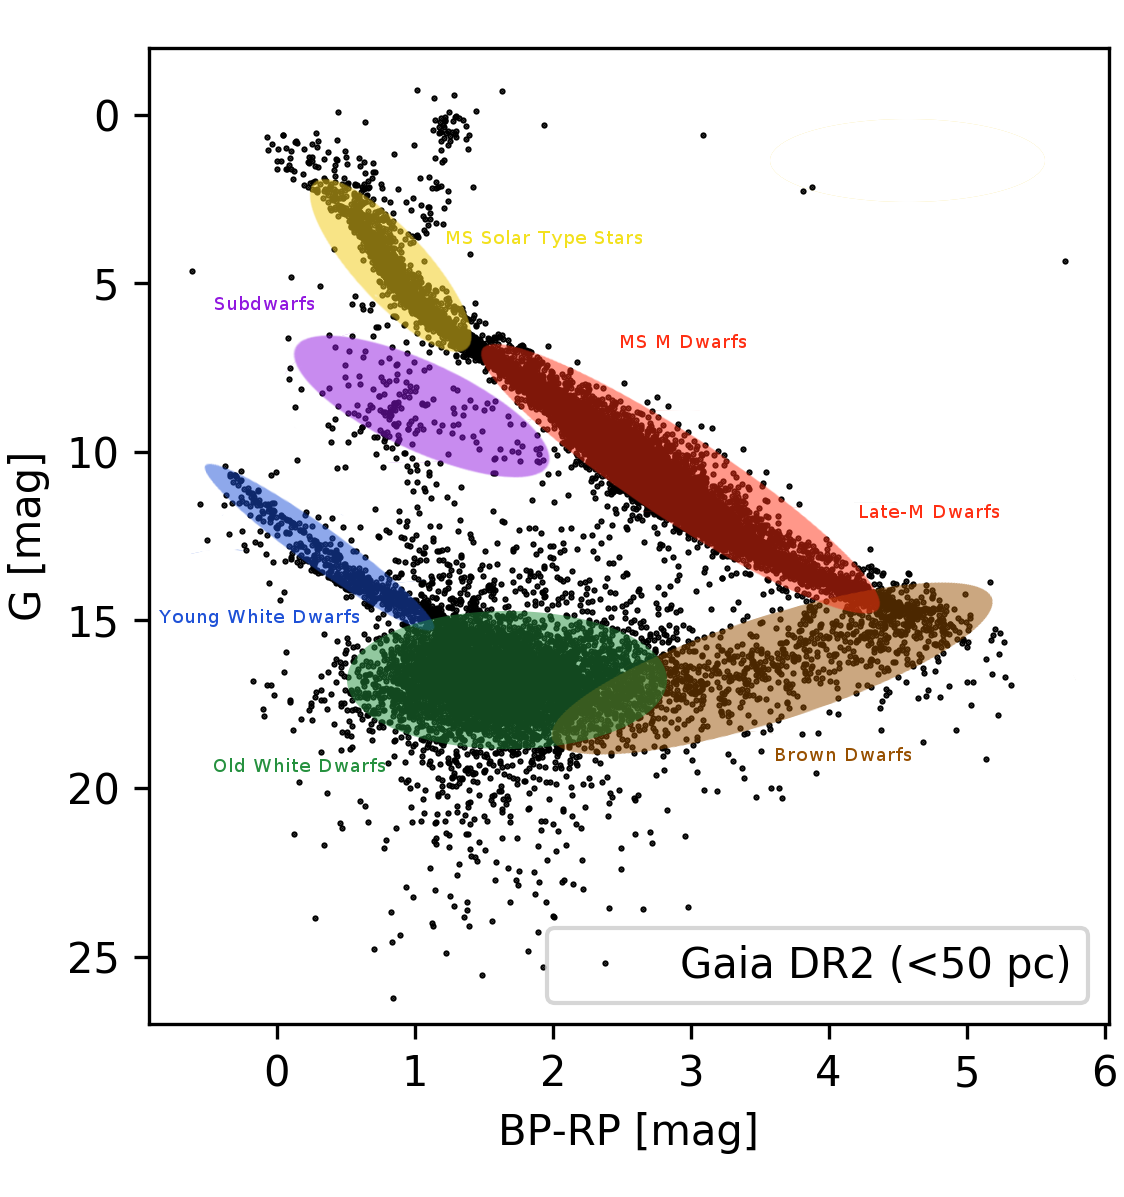
\includegraphics [scale=1] {gaia50types}
  \caption{На диаграмме <<показатель цвет B--R "--- абсолютная звездная величина в полосе G>> в величинах Gaia представлены звезды Gaia DR2 из ближайших окрестностей (до 50 пк). Цветными областями обозначено приблизительное разбиение звезд на группы, исходя из значений их показателей цвета и абсолютных звездных величин.}
  \label{fig:1}
\end{figure}

\begin{figure}[h]
  \centering
  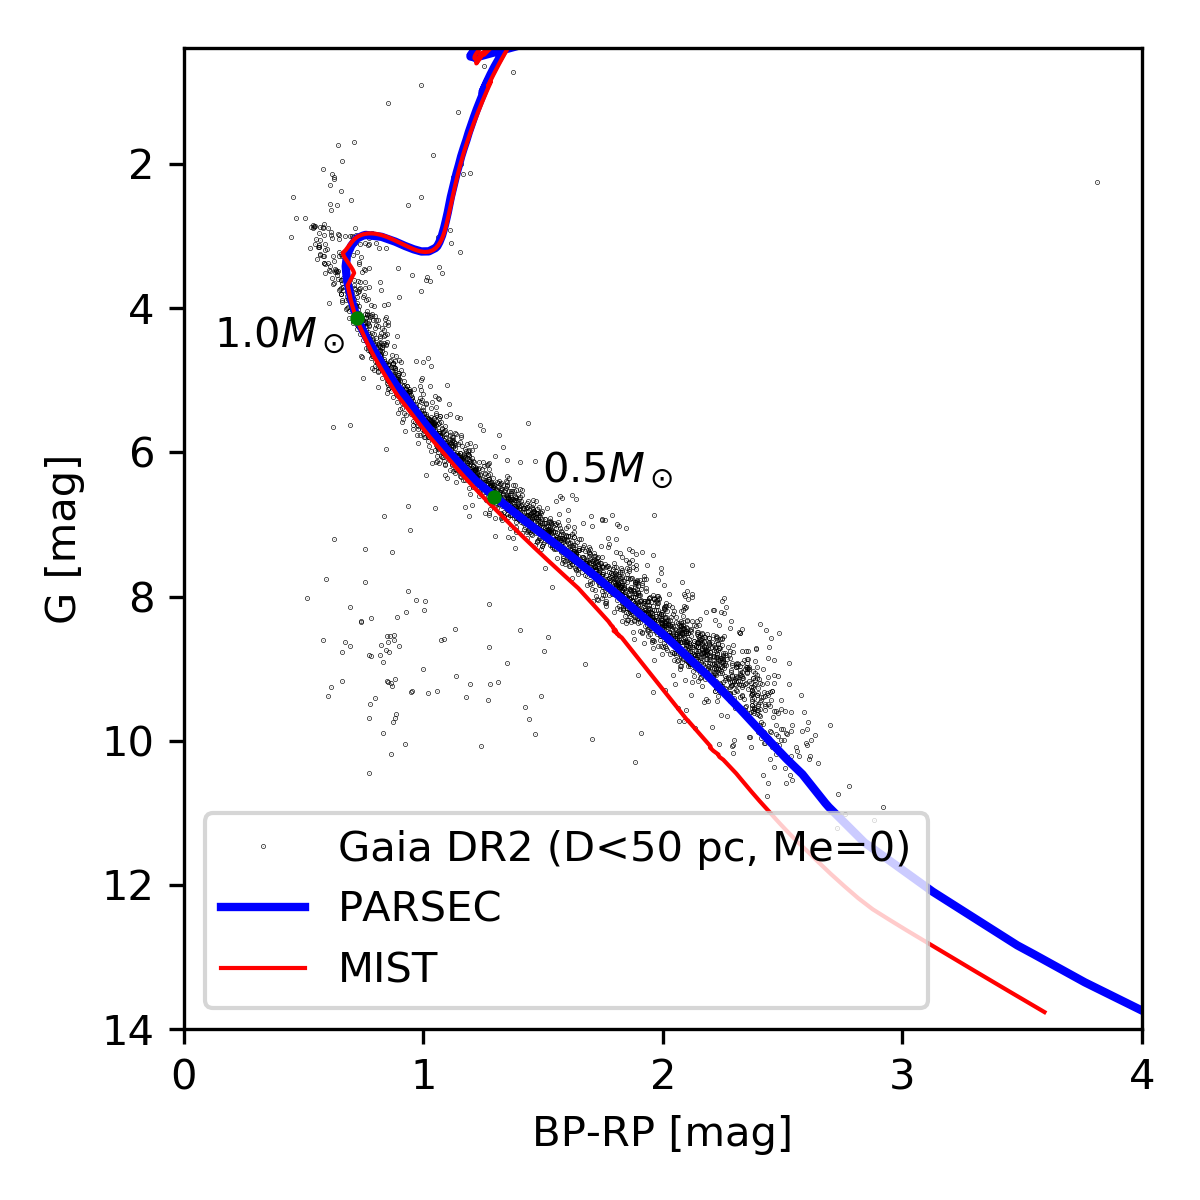
\includegraphics [scale=1] {parsec-mist-gaia}
  \caption{На диаграмме <<показатель цвета B--R "--- абсолютная звездная величина в полосе G>> в величинах Gaia представлены звезды Gaia DR2 из ближайших окрестностей (до 50 пк) с нулевой металличностью, соответствующие модельные изохроны проектов PARSEC и MIST, а также положения соответствующих звезд с массами 1 \(\textup{M}_\odot\) и 0.5 \(\textup{M}_\odot\).}
  \label{fig:2}
\end{figure}

В настоящее время существует ряд проектов, нацеленных на конструирование моделей звезд различных типов. На рис. 2 представлено сравнение звезд солнечной металличности из ближайших 50 пк по данным Gaia DR2 c модельными изохронами двух проектов: MIST (Choi et al., 2016) и PARSEC (Bressan et al., 2012). Как видно из рисунка, в то время, как для масс от 1 до 0.5 \(\textup{M}_\odot\) наблюдаемые данных очень хорошо согласуются с обеими изохронами, при массах менее 0.5 \(\textup{M}_\odot\) модели начинают значительное расхождение, причем согласие с наблюдениями в большей степени имеет изохрона PARSEC. Такое расхождение можно объяснить в большей степени эмпирическим характером построения той части модели, которая описывает менее массивные звезды. Авторы PARSEC отмечают, что такой подход прежде всего связан  с трудностью моделирования звездных атмосфер у объектов с сильным влиянием конвекционных процессов. Чтобы справиться с проблемой моделирования объектов легче 0.5 \(\textup{M}_\odot\), авторы PARSEC вносили поправки на основе наблюдаемых затменно--двойных звезд, для которых есть хорошие кривые лучевых скоростей (рис. 3). Однако, выяснилось, что наблюдаемые затменно--двойные звезды слишком тесные, и радиусы их компонент искажаются. Одно из предположений заключается в том, что в таких системах происходит инфляция радиуса за счёт взаимного нагрева компонент. Однако, попытка оценить такое влияние показала увеличение радиуса не более, чем на 6\,\%  при превосходстве светимости <<влияющего>> компаньона более, чем в 500 раз (рис. 4).



\begin{figure}[p]
  \begin{minipage}[ht]{1\linewidth}\centering
    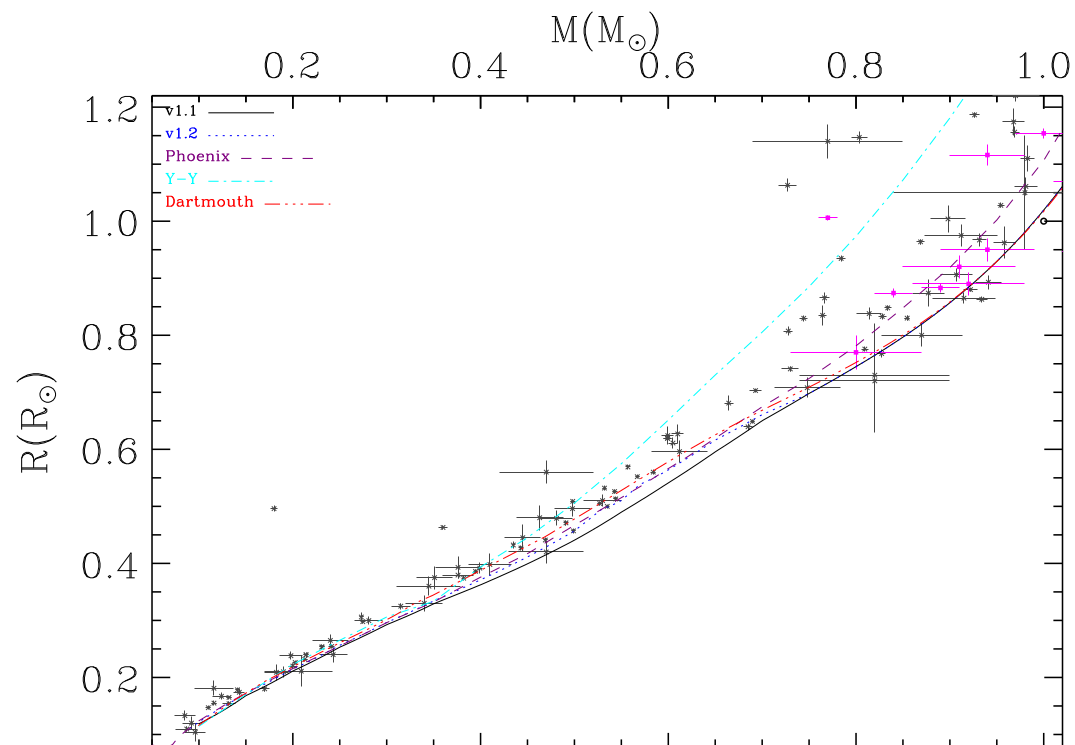
\includegraphics[width=0.8\linewidth]{parsecMRL1}% \\ а)
  \end{minipage}
  \hfill
  \begin{minipage}[ht]{1\linewidth}\centering
    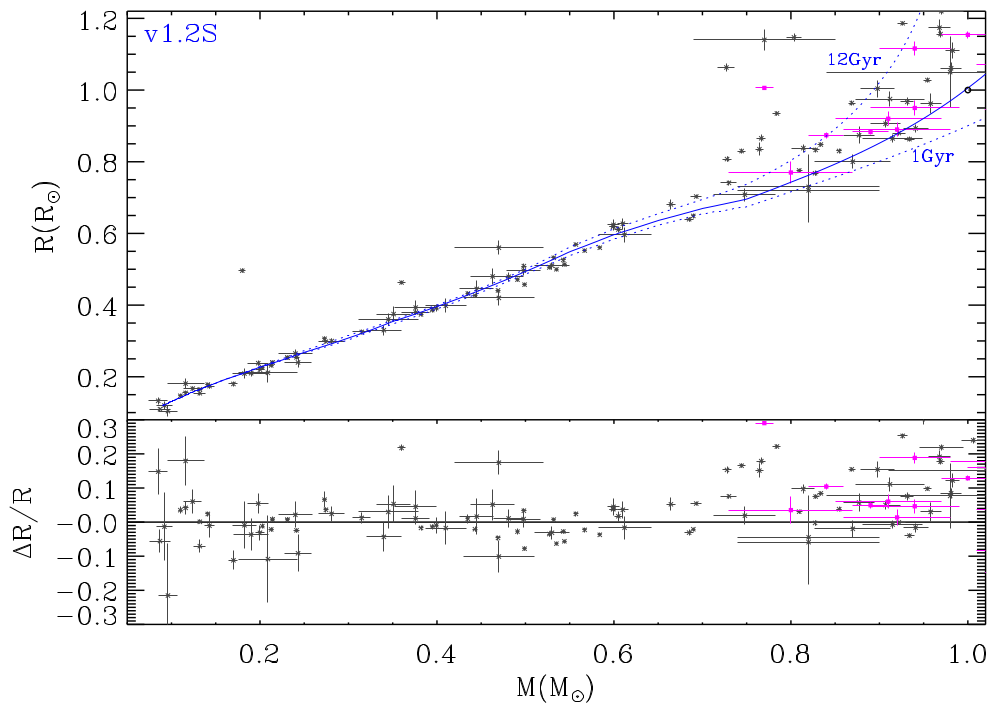
\includegraphics[width=0.775\linewidth]{parsecMRL2}% \\ б)
  \end{minipage}
  \caption{Сверху: эмпирическое отношение массы к радиусу для звезд с малой массой в солнечной окрестности. Черные звездочки -- это двойные звезды; пурпурные квадраты -- одиночные звезды. v1.1 и v1.2 -- версии изохрон PARSEC (версия 1.2 - уточненная при помощи наблюдений нескольких сотен затменно-двойных, для которых есть хорошие кривые лучевых скоростей). Снизу: то же, только построенное для откалиброванного отношения T-$\tau$ (T -- температура, $\tau$ -- средняя оптическая глубина Росселанда) и с добавление изоброн для возрастов 1Gyr и 12Gyr. Взято из Chen et al. (2014, рис. 2 и рис. 12).}
  \label{fig:3}
\end{figure}



\begin{figure}[h]
  \centering
  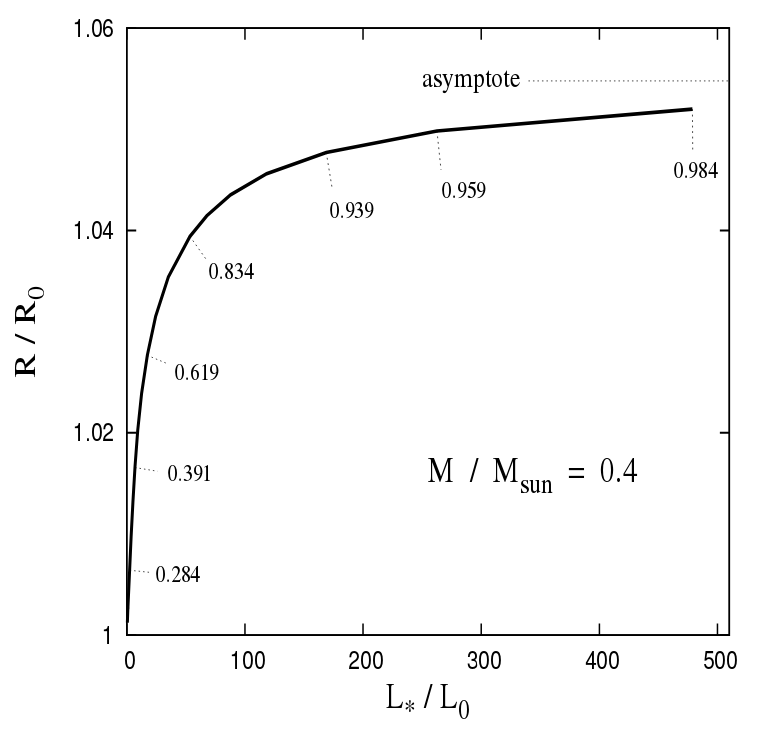
\includegraphics [scale=0.4] {radiusInflationLMSbinary}
  \caption{Попытка оценить влияние <<точечной>> компоненты затменно--двойной (a = 3 \(\textup{R}_0\)) со светимостью \(\textup{L}_*\) (отсечками на кривой показаны значения болометрического альбедо). Взято из Lucy (2018, рис. 4).}
  \label{fig:4}
\end{figure}

\begin{figure}[h]
  \centering
  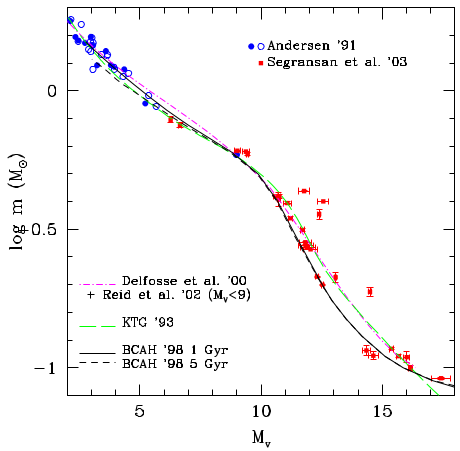
\includegraphics [scale=1] {chabrier-et-al-2005-3}
  \caption{Согласие теоретических моделей аналога зависимости <<масса "--- звёздная величина>> с наблюдаемыми данными. Заметоно расхождение теорий и наблюдений для звезд слабее 10 звездной величины и легче $\approx$0.5  \(\textup{M}_\odot\) (этому значению примерно соответствует отсчёт по вертикальной шкале около -0.3). Взято из Chabrier et al. (2005, рис. 3).}
  \label{fig:5}
\end{figure}

Упомянутая выше проблема учета конвекционных процессов в маломассивных звездах отмечается и в других работах. Например, в <<Обзоре маломассивных звезд и коричневых карликов>> (Chabrier et al. (2005)) говорится о сложности фотометрии звезд класса M5 и более поздних как раз из-за образования на поверхности большого числа звездных пятен и роста видимой активности диска и короны. Авторы объясняют это тем, что конвекция у таких объектов может распространяться вплоть до ядра.  Вообще, в данной работе говорится о целом наборе проблем, связанных с недостатком информации о карликах при их моделировании. На рис. 5 продемонстрировано, насколько хорошо существующие теоретические зависимости <<масса "--- абсолютная звездная величина>> согласуются с наблюдениями в оптическом диапазоне.

Как можно заметить, для звёзд до \(\textup{10}^m\) согласие достаточно хорошее, тогда как более слабые объекты по диаграмме распределены несколько более хаотично и сильнее отклоняются от гладких модельных кривых. В статье говорится, что, вероятно, это связано с образованием большого количество линий поглощения. Исследователи отмечают, что в атмосферах маломассивных звёзд и коричневых карликов образуется множество молекул, чьи конденсаты и частицы сильно влияют на тепловую непрозрачность этих атмосфер. Излучение молекул часто поглощается в оптическом диапазоне или слишком слабо из-за эффекта обратного нагрева верхних слоев, где линии формируются. Всё это приводит к видимому покраснению звёзд, в частности, коричневые карлики излучают до 90\,\% своей энергии в ИК полосах, и авторы называют наиболее перспективными исследования данных объектов именно в этом диапазоне. Однако, авторы доклада <<Необходимость инфракрасной астрометрии коричневых карликов в эпоху после Gaia>> (Kirkpatrick et al., 2019) указали на сложности наблюдений Gaia таких объектов. Исследователи отмечают, что диапазон наблюдений Gaia: $\lambda$ < 1,05 мкм (Gaia, 2016), поэтому подавляющее большинство коричневых карликов, чьи спектры достигают максимума в ИК, не могут быть обнаружены. Например, в ближайших 20 парсеках Gaia может полностью исследовать только типы $\approx$ L5 (Kirkpatrick et al. 2019a). И в материалах доклада проиллюстрирована необходимость астрометрического мониторинга на более длинных инфракрасных волнах.

Проблема надежного определения радиусов звёзд также упоминается в работе Шабрие (Chabrier et al., 2005). Отмечается, что используемые сейчас методы определения радиусов могут давать результаты, сильно отличающиеся друг от друга. Значения радиусов, определяемые через оценку наклона кривой блеска у затменных двойных получаются в среднем в 2 раза больше аналогичных радиусов, определенных высокоточной интерферометрией или через эффект графитационного линзирования. Как уже отмечалось выше, это может быть связано с эффектом взаимного нагрева слишком тесных систем.

Имеет смысл упомянуть об исследованиях по построению и интерпретации функции масс в окрестностях границы <<звёзды "--- коричневые карлики>>, данная проблема также является проблемной  (см., например, Тис и др., 2015).  Кроме того, отмечается, что космогонические модели помогают выделять наиболее вероятные сценарии формирования и эволюции звёздных популяций (Тис и др., 2015), однако они нуждаются в постоянном уточнении и сравнении с наблюдательными данными.

В качестве очередного примера попытки построения эмпирической MLR можно отметить работу Eker et al. (2018), где использовались наблюдения звезд с наиболее надежными массами и светимостями. Всего в работу вошло 55 маломассивных объектов. На рис. 6 представлено сравнение этой модели с аналогичными моделями упомянутых проектов  MIST и PARSEC, и как можно заметить, модели начинают расходиться при светимости меньше 0.1 \(\textup{L}_\odot\), а наблюдаемые в пулковской программе звезды (Shakht et al., 2018) лежат у границ погрешности модели Eker et al. (2018), обозначенных пунктирной линией. Это может быть связано с тем, что для звезд M < 0.7 \(\textup{M}_\odot\) имеет место острый дефицит надежно определенных масс, а калибровка существующих моделей карликовых звезд привязана к тесным системам, где оценки M и L могут быть искажены систематическими ошибками (несферичность, взаимный нагрев).

\begin{figure}[h]
  \centering
  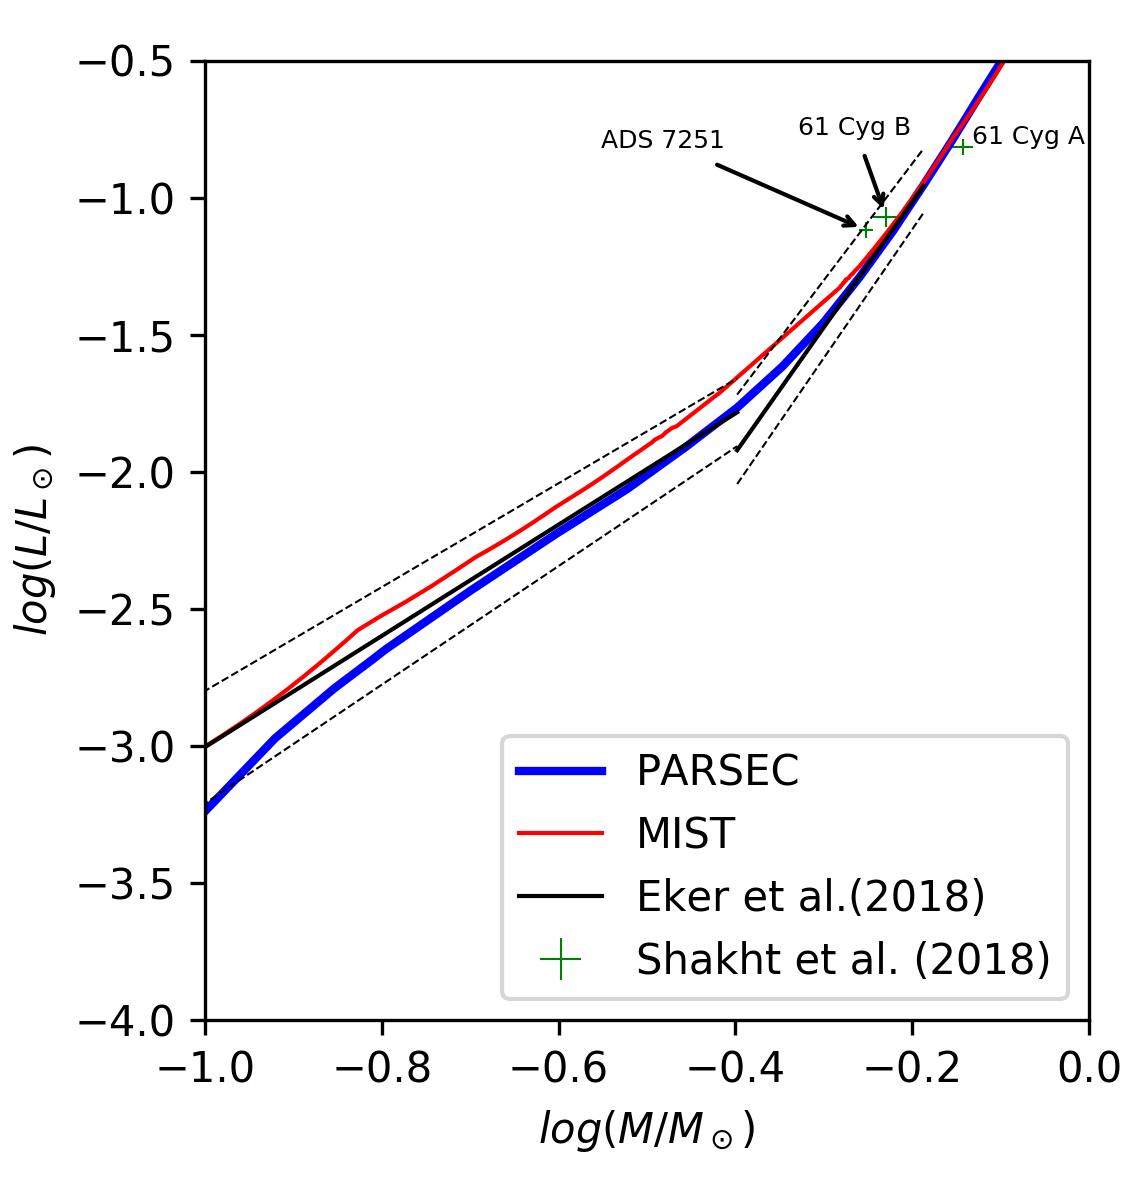
\includegraphics [scale=1] {mass-lum}
  \caption{Эмпирическая модель MLR Eker et al. (2018) (пунктиром обозначена граница ошибок модели), а также  аналогичные модели проектов PARSEC и MIST. Крестами обозначены визуально-двойные звезды из пулковской программы (Shakht et al. (2018)).}
  \label{fig:6}
\end{figure}

Возможным решением части указанных проблем могут служить исследования различных типов двойных и кратных систем карликов, в том числе "--- более широких, порядок периодов которых с одной стороны позволяет строить взаимные орбиты по высокоточным длительным наблюдениям, а с другой стороны "--- пространственное разделение компонент позволяло бы рассматривать каждую из компонент как одиночную звезду, без значительного влияния компаньона (большие полуоси у таких систем составляют порядка 10 а.е.). В современной науке можно найти многочисленные примеры работ, посвященных поиску, разделению компонент и построению орбит двойных систем  (см., например, Кортес и др., 2015; Опитц и др., 2016) или по крайней мере отмечающие важность таких исследований.  

Построение исленных модели процессов звездообразования, эволюции и распределения свойств объектов легче 0.5 \(\textup{M}_\odot\) из молекулярных облаков позволяет подойти к проблеме оценки искомых статистических величин со стороны, противоположной сбору эмпирических данных, и  также является актуальной задачей. Сейчас можно найти ряд работ, посвященных этой теме. Например, в работе Bate (2019) представлен пример симуляции процесса формирования звездного скопления. В данной работе учитываются химический состав межзвездной среды, влияние космических лучей, нагрев газа и пыли из-за излучения звезд, процессы диффузии и переноса излучения. В итоге модельное облако M = 500 \(\textup{M}_\odot\) порождает порядка сотни звезд суммарной массы $\approx$ 100 \(\textup{M}_\odot\) с медианной массой 0,15 \(\textup{M}_\odot\). Как видно из рис. 7, получившаяся функция масс наилучшим образом согласуется с результатами построения IMF Chabrier (2005), собравшим наблюдения маломассивных звезд и коричневых карликов на протяжении 50 лет.  Особое место в исследовании отведено изучению доли и свойств кратных объектов. Как следует из рис. 8, доля кратных систем в получившейся модели растёт с увеличением начальных масс объектов, и этот результат подтверждают и эмпирические данные. Причем исследователи отмечают, что так как доля кратных систем имеет явную корреляцию с значениями начальных масс, то при сравнении моделирования с наблюдениями всегда стоит использовать аналогичные диапазоны масс. На рис. 9 представлено сравнение получившейся гистограммы распределения двойных, тройных и четверных систем по большим полуосям (тройные системы дают два значения полуосей, а четверные "--- три) с двумя эмпирическими моделям: для M--карликов и звезд с начальными массами солнечного типа. Отмечается, что поскольку большинство моделируемых объектов имеют малую массу, то ожидается, что распределение для M--карликов должно лучше соответствовать модели, и этот результат в большей мере воспроизводит гистограмма для двойных систем.  

\begin{figure}[h]
  \centering
  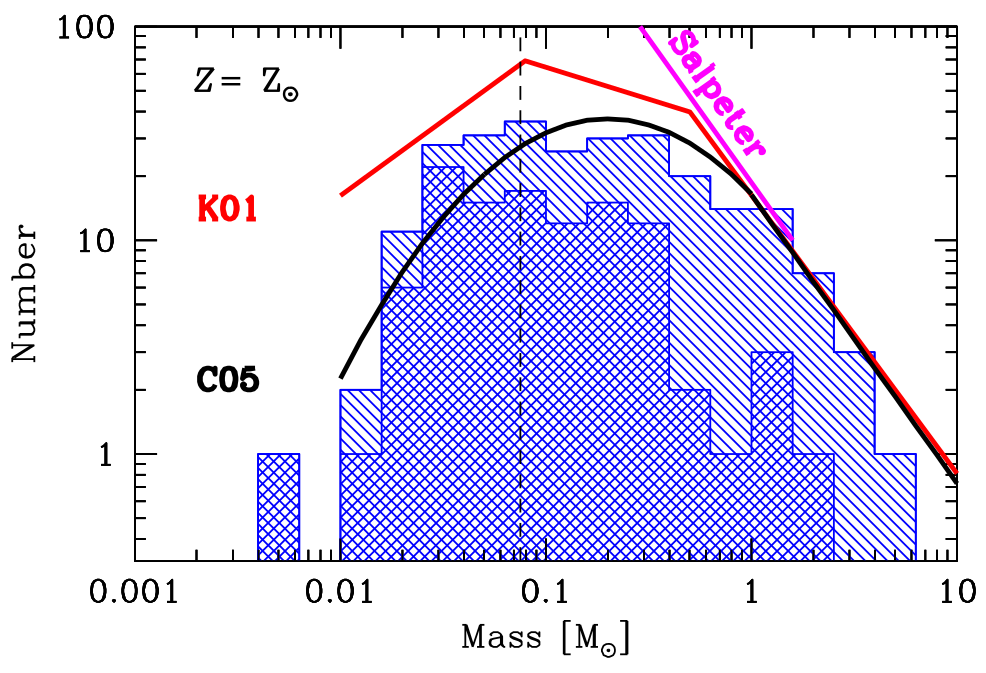
\includegraphics [scale=0.4] {Bate-IMF}
  \caption{Гистограмма IMF звезд и коричневых карликов солнечной металличности в рамках численной модели Bite (2009). Двойная штриховка - объекты без аккреции, одиночная штриховка - с аккрецией. Функции масс хорошо согласуются с данными Chabrier (2005) (С05). Также представлены две другие IMF: Salpeter (1955) и Kroupa (2001). Взято из Bate (2019, рис. 8, нижний левый).}
  \label{fig:7}
\end{figure}

\begin{figure}[h]
  \centering
  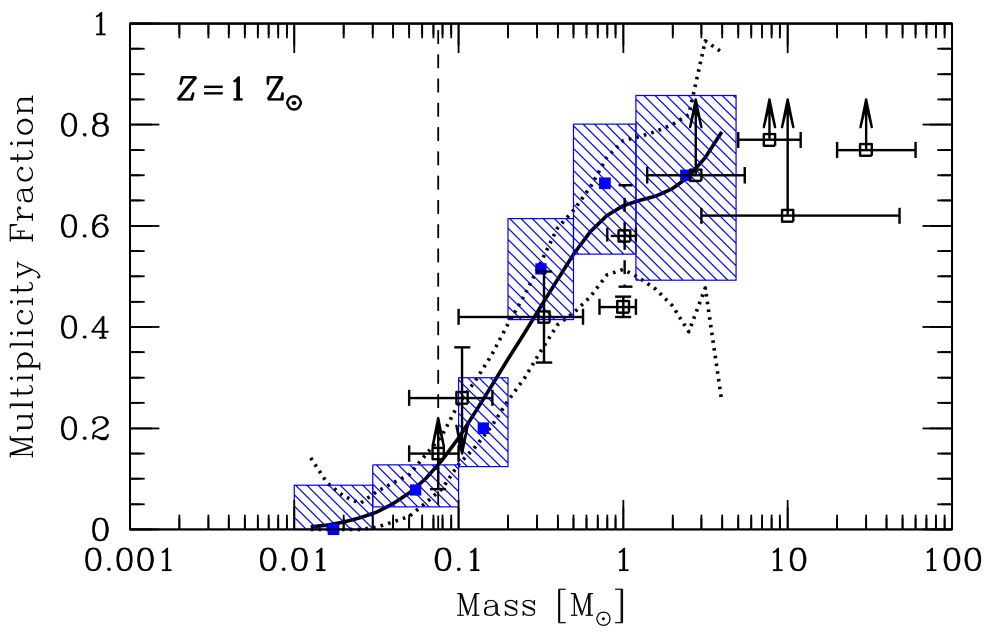
\includegraphics [scale=0.4] {Bate-BF}
  \caption{Доля кратности в зависимости от первичной массы звезд солнечной металличности в рамках численной модели Bite (2009). Синие закрашенные квадраты, окруженные заштрихованными областями, представляют результаты численных расчетов со статистической погрешностью 1$\sigma$. Толстая сплошная линия - кривая долей кратности, вычисленная с использорванием скользящего логарифма, пунктирные линии - на 1$\sigma$--интервале вокруг нее. Незакрашенные квадраты с погрешностями и пределами - наблюдаемые доли кратных из исследований  Close et al. (2003), Basri and Reiners (2006), Fischer and Marcy (1992), Raghavan et al. (2010), Duquennoy and Mayor (1991), Kouwenhoven et al. (2007), Rizzuto et al. (2013), Preibisch et al. (1999) and Mason et al. (1998) слева направо.  Исследователи отмечают, что наблюдаемая тенденция увеличения кратности воспроизводится всеми рассмотренными расчетами, и поскольку доля кратных сильно зависит от начальных масс, важно, чтобы при сравнении моделей с наблюдениями использовались аналогичные массы. Взято из Bate (2019, рис. 10, нижний левый).}
  \label{fig:8}
\end{figure}

\begin{figure}[h]
  \centering
  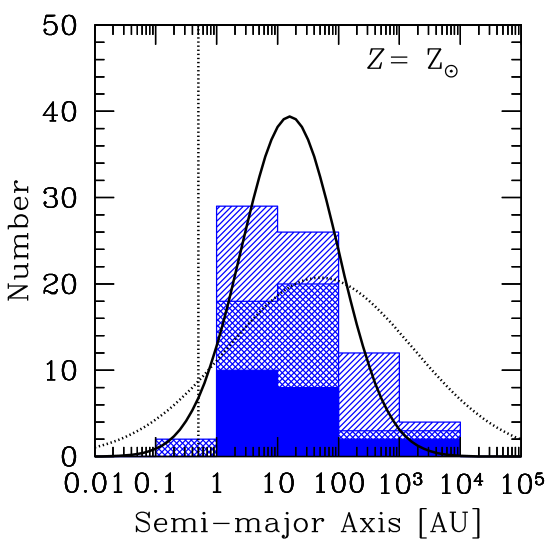
\includegraphics [scale=0.6] {Bate-a-distr}
  \caption{Гистограмма распределения кратных звезд солнечной металличности с начальными массами > 0.1Msun по большим полуосям в рамках численной модели Bite (2009).  Бары с одиночной, двойной и сплошной штриховкой представляют двойные, тройные и четверные системы соответственно. Сплошная кривая - распределение M-карликов из обзора Janson et al.(2012), а пунктирная - распределение звезд с начальными массами солнечного типа из обзора Raghavan et al. (2010). Поскольку большинство моделируемых систем имеют малую массу, ожидается, что распределение Janson et al. будет соответствовать лучше, чем Raghavan et al. Вертикальная пунктирная линия показывает предел разрешающей способности расчетов, который определяется радиусами аккреции поглощающих частиц (0,5 а.е.). Взято из Bate (2019, рис. 11, третий слева).}
  \label{fig:9}
\end{figure}

Попытка воссоздания эволюции доли двойных систем для кластеров звезд с различными начальными параметрами представлена, например, в работе Hurley et al., 2007. На рис. 10 представлен результат моделирования эволюции доли двойных систем в кластере из 100 000 звезд, где в начальный заданный момент времени доля двойных составляла 10\,\%. Из рисунка видно, что с течением времени прогнозируемое моделью число кратных систем имеет явный тренд к возрастанию.

\begin{figure}[h]
  \centering
  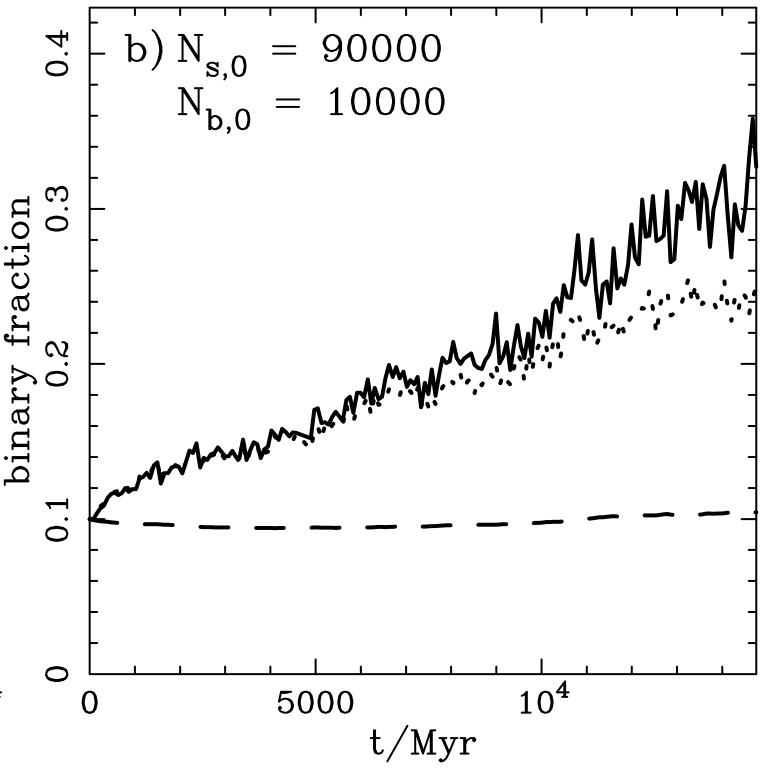
\includegraphics [scale=0.4] {Hurley}
  \caption{Эволюция доли двойных систем в ядре (сплошная линия), в пределах 10\% радиуса Лагранжа (пунктирная линия) и для всего кластера (пунктирная линия) в одной из моделей. Ns,0 Nb,0 -  количества одинарных и двойных звезд в исходной модели.  Взято из Hurley et al. (2007, рис. 7b).}
  \label{fig:10}
\end{figure}

Однако, пока сложно утверждать, что даже совокупность существующих обзоров и программ решает проблему в полной мере. К сожалению, несмотря на существенный прогресс в исследовании кратных систем, который дает Gaia DR2, даже после значительного исправления первого релиза, данные миссии также не имеют полноты выборки для визуальных двойных звезд с разделением $\rho$ менее $2''$ (рис.11), что отмечают и авторы (Арно и др., 2018; Линдерген и др., 2018). Это может быть связано со сложностью анализа изображения тесных систем в Gaia DR2 (Fabricius et al., 2016), когда FWHM (ширина на полувысоте) становится меньше $\rho$ (см. рис. 12). Сложность разделения тесных систем сказывается и на ошибках определения пиксельных координат, что в свою очередь влияет на вычисляемые значения собственных движений и параллаксов. Например, на рис. 13 можно увидеть, как относительная точность параллаксов Gaia DR2 падает при $\rho$ < $2''$. Кроме того, отмечается проблема кросс--идентификации быстрых объектов ($\mu$ > 100 mas/yr), которые в основном как раз относятся к ближайшему звездному населению. Как указано в GaiaDR2 Documentation 1.2 (2019), для звезд с разделением менее $0.7''$ всегда будет стоять проблема кросс--идентификации, и поэтому объекты GaiaDR2 с флагом <<duplicate source>> предлагается отдельно проверять, являются ли они действительно дубликатами одинокой звезды или же входят в кратную систему. Помимо проблемы отождествления тесных объектов, стоит упомянуть, что период наблюдений миссии Gaia строго ограничен и не дает возможности получения достаточного количества наблюдений для построения орбит широких пар, периоды взаимного обращения которых сильно превалируют над сроком жизни спутника.

\begin{figure}[h]
  \centering
  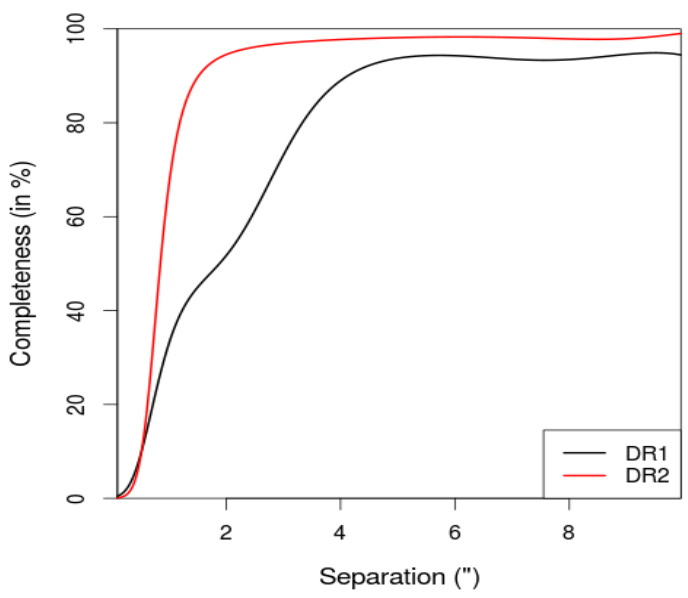
\includegraphics [scale=0.5] {gaia-complitness-for-binaries}
  \caption{Полнота (\%) визуальных двойных звёзд из каталога WDS в зависимости от разделения между компонентами (WDS), детектируемых в ходе миссии Gaia.  Gaia DR1 (черный), Gaia DR2 (красный). Заметно снижение полноты выборки двойных для тесных систем ($\rho$ < 2 arcsec). Взято из Arenou et al. (2018, рис. 8).}
  \label{fig:11}
\end{figure}

\begin{figure}[h]
  \centering
  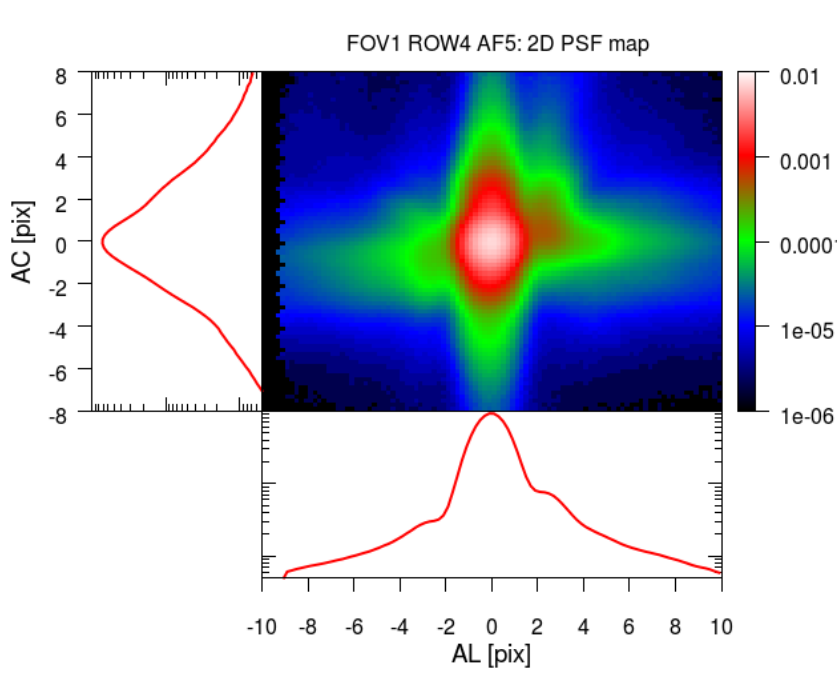
\includegraphics [scale=0.5] {gaia-psf}
  \caption{PSF изображения тесной двойной (1.2arcsec на 2.8arcsec) демонстрирует сложность разделения в Gaia DR2 изображений подобных звезд. Взято из Fabricius et al. (2016,  рис. 7).}
  \label{fig:12}
\end{figure}

\begin{figure}[h]
  \centering
  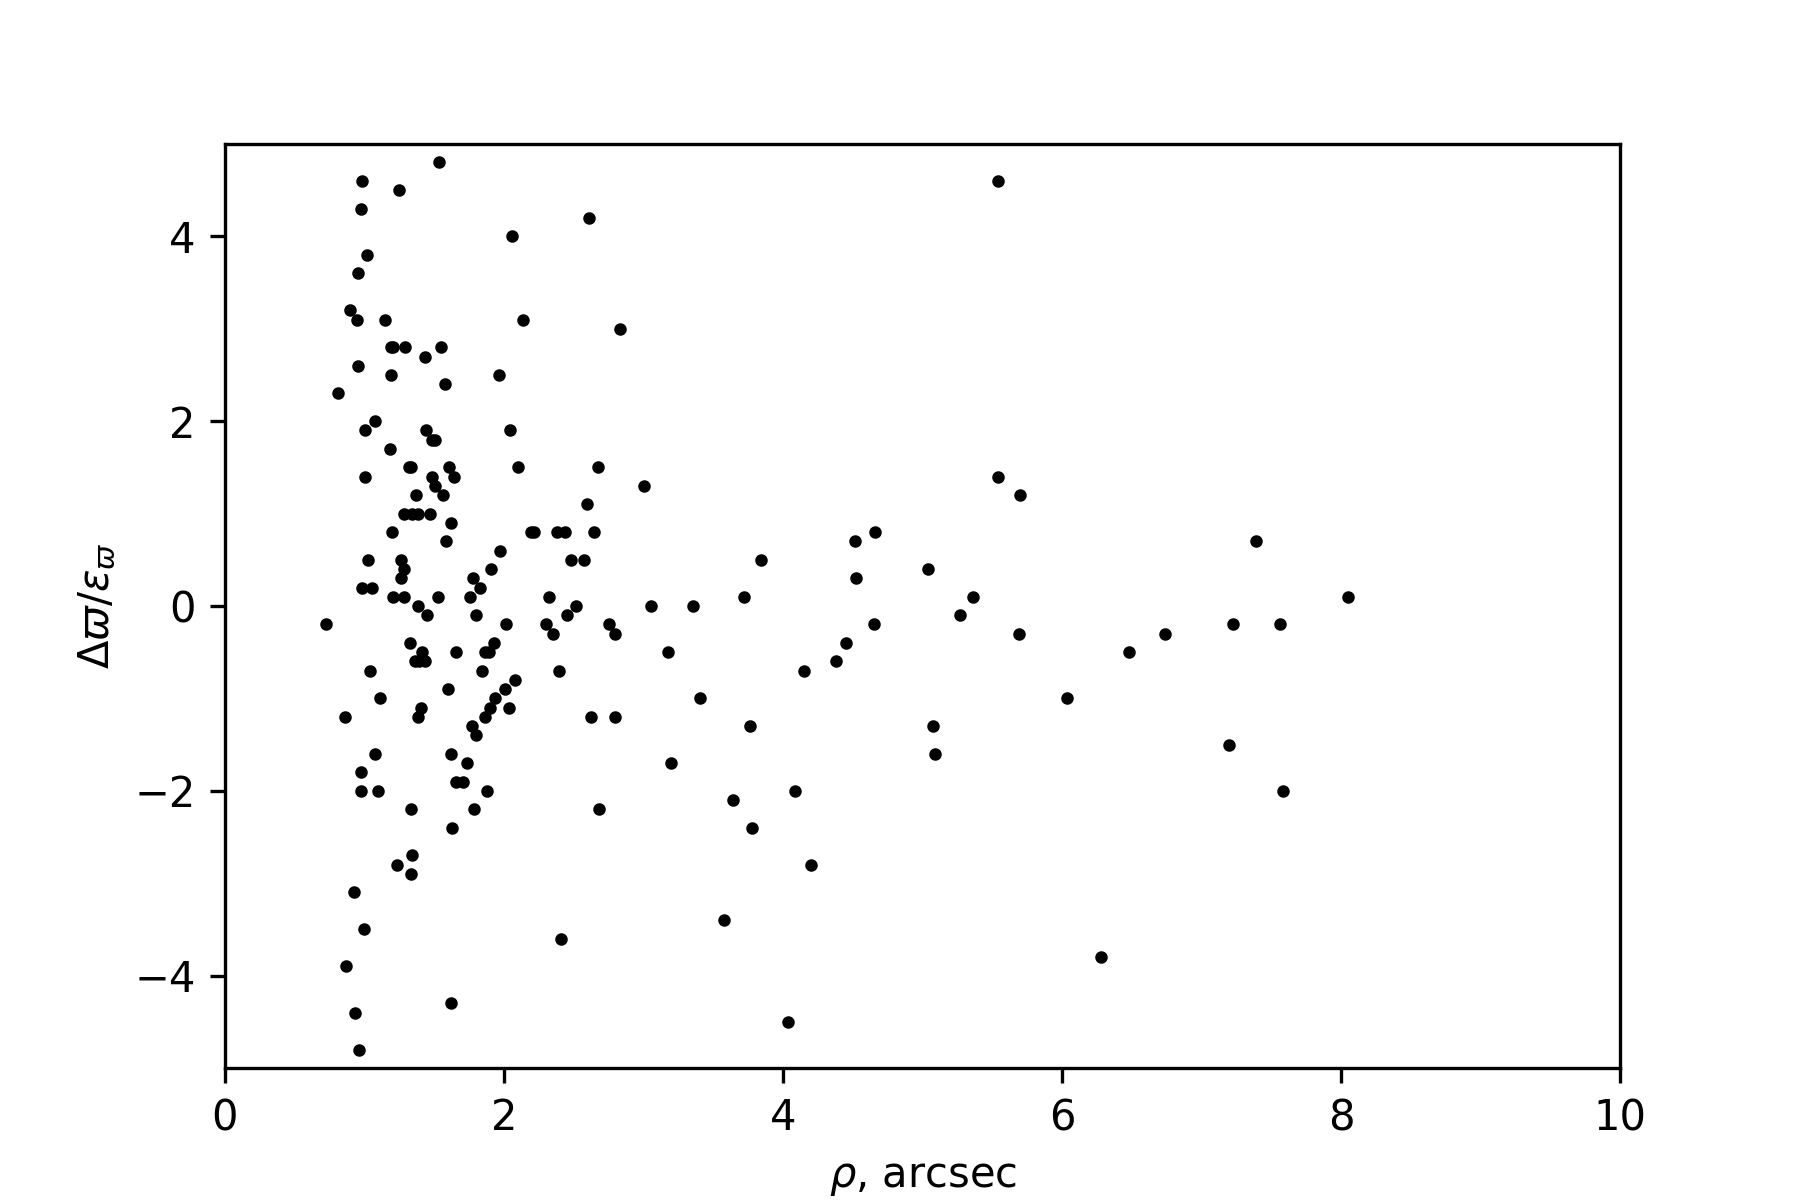
\includegraphics [scale=1] {delta_pi-vs-rho}
  \caption{Увеличение разброса относительных ошибок параллаксов Gaia для изображений звезд с разделением менее 3 arcsec указывает на существенное снижение точности определения пиксельных координат компонент.}
  \label{fig:13}
\end{figure}

В связи с указанными проблемами важным становится применение всех доступных методик детектирования кратности звезд и использование по возможности всех доступных наблюдений звезд, охватывающих широкий диапазон эпох. Исследования звезд в ближайших 50 пк от Солнца дают возможность наиболее эффективного их применения. Как можно убедиться из рис.  14, для звездных систем с величинами больших полуосей порядка 10 а.е. видимое разделение компонент даже в ближайшем окружении составляет меньше $1''$. К счастью, существующие методы высокого разрешения (спекл--интерферометрия, Lucky images) позволяют разделять объекты с $\rho$ < $1''$ (см. рис. 15). Однако данные методы сложно применять массово, так как требуют таргетированных и часто многочисленных наблюдений, и больше подходят для построения орбит уже выявленных двойных и кратных систем.

\begin{figure}[h]
  \centering
  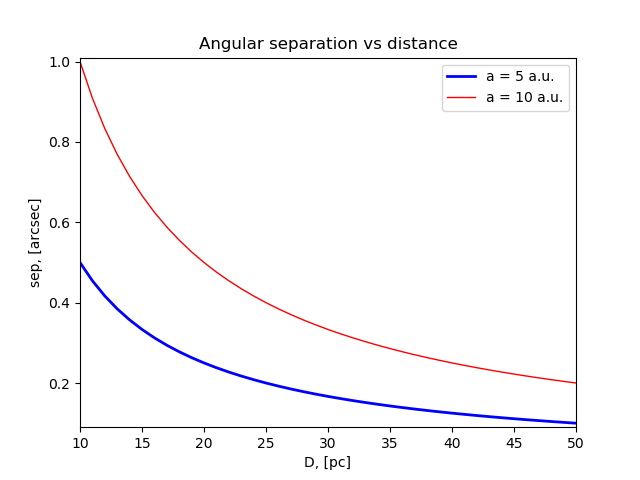
\includegraphics [scale=1] {separation-vs-distance}
  \caption{Поиск и определение динамических параметров маломассивных двойных систем – актуальная задача для наблюдателей. Для широкого класса подобных объектов $\rho$ < FWHM.}
  \label{fig:14}
\end{figure}

\begin{figure}[h]
  \centering
  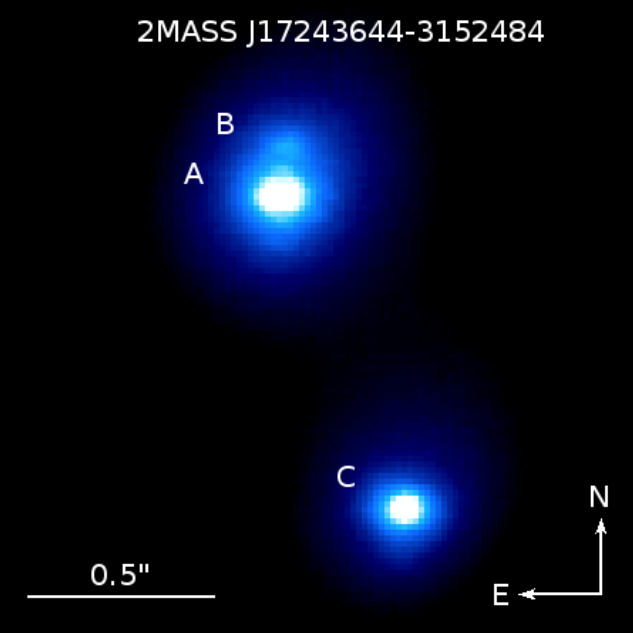
\includegraphics [scale=0.5] {lucky-imaging-example}
  \caption{Рис 15. 3.5m New Technology Telescope (NTT) - метод удачных экспозиций (Lucky images). Взято из Janson et al. (2017, рис. 1). }
  \label{fig:15}
\end{figure}

Близость исследуемых объектов позволяют эффективно применять различные методы современной астрономии для их изучения. Например, наиболее заметные смещения компонент близких систем по лучу зрения дают возможность плодотворно выявлять оптически неразрешаемые спектрально-двойные звезды благодаря значительному проявлению эффекта доплеровского смещения спектральных линий и сокращению влияния поглощения излучения межзвездной средой. Однако, объектами таких исследований становятся в основном всё те же тесные системы, массы и радиусы которых сложно использовать для построения моделей одиночных звезд.

Целью данной работы является разработка метода поиска двойных и кратных звезд, наблюдения орбит которых позволят получить более надежные массы, радиусы и светимости маломассивных звезд и коричневых карликов и уточнить фундаментальные закономерности для этих групп объектов. Исследуемые системы преимущественно должны быть не слишком тесными, чтобы компоненты не влияли в значительной мере на характеристики друг друга, а их периоды позволяли бы построить орбиты для получения масс компонент. Поэтому объекты для таких целей представляют собой в среднем двойные звезды низкой светимости из ближайшего окружения Солнца, большие полуоси взаимных орбит которых составляют примерно 5"---10 а.е.. Даже в ближайшем окружении такие системы часто разрешимы только  с помощью наблюдений методами высокого разрешения  (спекл--интерферометрия, Lucky images), которые нельзя использовать для массовых наблюдений. А современная наука в связи с развитием техники требует обработки всё большего объема информации и это вынуждает ученых создавать хорошо алгоритмизируемые методы исследования.

С учетом специфики объектов (высокие собственные движения за счёт малого расстояния) в целях массовых исследований и выявления наиболее перспективных кандидатов в двойные звезды был выбран астрометрический анализ собственных движений. Отличительной характеристикой  такого анализа является то, что он не требует большого числа высокоточных современных наблюдений одних и тех же объектов, однако использует в совокупности с доступными современными наблюдениями и наиболее ранние наземные, что обеспечивает высокую точность определения собственных движений даже при значительных ошибках положений звезд. Это дало возможность на раннем этапе отладки методики использовать собственные наблюдения Пулковской обсерватории, анализ изображений которых открыл дополнительный метод детектирования кратности звезд "--- по анализу формы изображения звезды. По данной теме также была изучена теоретическая база и данный метод также был апробирован совместно с спекл--интерферометрическими исследованиями.

Двухэтапный подход и применение всех доступных наблюдений выгодно отличает исследуемый в данной работе метод. С одной стороны хорошо алгоритмизируемые методы астрометрического отбора позволяют обрабатывать на первом этапе большие объемы информации. А с другой "--- второй этап позволяет убедиться в точности проведенных исследований и подтвердить открытия, сделанные в результате первой части исследования.

В ходе апробации описанных выше методов были выявлены ранее неизвестные двойные и тройные системы. Для одной из звезд в настоящее время ведутся наблюдения для построения орбиты.

\newpage
*********************************************

Дальше "--- то, что предлагает форма с github.
% {\progress}
% Этот раздел должен быть отдельным структурным элементом по
% ГОСТ, но он, как правило, включается в описание актуальности
% темы. Нужен он отдельным структурынм элемементом или нет ---
% смотрите другие диссертации вашего совета, скорее всего не нужен.

{\aim} данной работы является \ldots

Для~достижения поставленной цели необходимо было решить следующие {\tasks}:
\begin{enumerate}
  \item Исследовать, разработать, вычислить и~т.\:д. и~т.\:п.
  \item Исследовать, разработать, вычислить и~т.\:д. и~т.\:п.
  \item Исследовать, разработать, вычислить и~т.\:д. и~т.\:п.
  \item Исследовать, разработать, вычислить и~т.\:д. и~т.\:п.
\end{enumerate}


{\novelty}
\begin{enumerate}
  \item Впервые \ldots
  \item Впервые \ldots
  \item Было выполнено оригинальное исследование \ldots
\end{enumerate}

{\influence} \ldots

{\methods} \ldots

{\defpositions}
\begin{enumerate}
  \item Первое положение
  \item Второе положение
  \item Третье положение
  \item Четвертое положение
\end{enumerate}
В папке Documents можно ознакомиться в решением совета из Томского ГУ
в~файле \verb+Def_positions.pdf+, где обоснованно даются рекомендации
по~формулировкам защищаемых положений.

{\reliability} полученных результатов обеспечивается \ldots \ Результаты находятся в соответствии с результатами, полученными другими авторами.


{\probation}
Основные результаты работы докладывались~на:
перечисление основных конференций, симпозиумов и~т.\:п.

{\contribution} Автор принимал активное участие \ldots

\ifnumequal{\value{bibliosel}}{0}
{%%% Встроенная реализация с загрузкой файла через движок bibtex8. (При желании, внутри можно использовать обычные ссылки, наподобие `\cite{vakbib1,vakbib2}`).
    {\publications} Основные результаты по теме диссертации изложены в XX печатных изданиях,
    X из которых изданы в журналах, рекомендованных ВАК,
    X "--- в тезисах докладов.
}% 
{%%% Реализация пакетом biblatex через движок biber
    \begin{refsection}[bl-authorvak,bl-authorwos,bl-authorscopus,bl-authorother,bl-authorconf]
        % Это refsection=1.
        % Процитированные здесь работы:
        %  * подсчитываются, для автоматического составления фразы "Основные результаты ..."
        %  * попадают в авторскую библиографию, при usefootcite==0 и стиле `\insertbiblioauthor` или `\insertbiblioauthorgrouped`
        %  * нумеруются там в зависимости от порядка команд `\printbibliography` в этом разделе. 
        %  * при использовании `\insertbiblioauthorgrouped`, порядок команд `\printbibliography` в нём должен быть тем же (см. biblio/biblatex.tex)
        %
        % Невидимый библиографический список для подсчёта количества публикаций:
        \printbibliography[heading=nobibheading, section=1, env=countauthorvak,    keyword=biblioauthorvak]%
        \printbibliography[heading=nobibheading, section=1, env=countauthorwos,    keyword=biblioauthorwos]%
        \printbibliography[heading=nobibheading, section=1, env=countauthorscopus, keyword=biblioauthorscopus]%
        \printbibliography[heading=nobibheading, section=1, env=countauthorconf,   keyword=biblioauthorconf]%
        \printbibliography[heading=nobibheading, section=1, env=countauthorother,  keyword=biblioauthorother]%
        \printbibliography[heading=nobibheading, section=1, env=countauthor,       keyword=biblioauthor]%
        %
        % Цитирования.
        %  * Порядок перечисления определяет порядок в библиографии (только внутри подраздела, если `\insertbiblioauthorgrouped`).
        %  * Если не соблюдать порядок "как для \printbibliography", нумерация в `\insertbiblioauthor` будет кривой.
        %  * Если цитировать каждый источник отдельной командой --- найти некоторые ошибки будет проще.
        %
        %% authorvak
        \nocite{vakbib1}%
        \nocite{vakbib2}%
        %
        %% authorwos
        \nocite{wosbib1}%
        %
        %% authorscopus
        \nocite{scbib1}%
        %
        %% authorconf
        \nocite{confbib1}%
        \nocite{confbib2}%
        %
        %% authorother
        \nocite{bib1}%
        \nocite{bib2}%
        %
        %
        {\publications} Основные результаты по теме диссертации изложены в~\arabic{citeauthor}~печатных изданиях,
        \newcounter{citeauthorscwostot}% сумма citeauthorscopus и citeauthorwos
        \setcounter{citeauthorscwostot}{\value{citeauthorscopus}}%
        \addtocounter{citeauthorscwostot}{\value{citeauthorwos}}%
        \arabic{citeauthorvak} из которых изданы в журналах, рекомендованных ВАК\sloppy%
        \ifnum \value{citeauthorscwostot}>0%
            , \arabic{citeauthorscwostot} "--- в~периодических научных журналах, индексируемых Web of Science и Scopus\sloppy%
        \fi%
        \ifnum \value{citeauthorconf}>0%
            , \arabic{citeauthorconf} "--- в~тезисах докладов.
        \else%
            .
        \fi
    \end{refsection}%
    \begin{refsection}[bl-authorvak,bl-authorwos,bl-authorscopus,bl-authorother,bl-authorconf]
        % Это refsection=2.
        % Процитированные здесь работы:
        %  * попадают в авторскую библиографию, при usefootcite==0 и стиле `\insertbiblioauthorimportant`.
        %  * ни на что не влияют в противном случае
        \nocite{vakbib2}%vak
        \nocite{bib1}%other
        \nocite{confbib1}%conf
    \end{refsection}%
	%
	% Всё, что вне этих двух refsection, это refsection=0,
	%  * для диссертации - это нормальные ссылки, попадающие в обычную библиографию
	%  * для автореферата:
	%     * при usefootcite==0, ссылка корректно сработает только для источника из `external.bib`. Для своих работ --- напечатает "[0]" (и даже Warning не вылезет).
	%     * при usefootcite==1, ссылка сработает нормально. В авторской библиографии будут только процитированные в refsection=0 работы.
}

При использовании пакета \verb!biblatex! для автоматического подсчёта
количества публикаций автора по теме диссертации, необходимо
их~перечислить с использованием команды \verb!\nocite! в \verb!common/characteristic.tex!
